\section{Frameworks}

Im Umfeld des Machine Learnings sind zahlreiche Frameworks für verschiedene Plattformen und verschiedene Sprachen zu
finden. Diese sind auf unterschiedlichen Abstraktionsebenen angesiedelt und dementsprechend unterschiedlich komplex
in der Verwendung.
Je höher ein Framework dabei angesiedelt, desto einfacher ist es üblicherweise zu bedienen, bietet dem Anwender aber
dafür nur sehr stark eingeschränkte Möglichkeiten. Frameworks hingegen, die auf einem niedrigen Level operieren, bieten
dem Anwender sehr detaillierte und komplexe Möglichkeiten, den gesamtem Programmfluss zu beeinflussen, sind dadurch aber
auch deutlich komplexer zu verwenden.
Die Frameworks sind insbesondere darauf ausgerichtet, eine Implementation für die konkreten mathematischen Berechnungen
und Modelle zu bieten, die darüber hinaus auch hinsichtlich der Performance optimiert worden sind.

Zu nennen wären beispielsweise die nachfolgenden drei Frameworks:

\begin{enumerate}
    \item{Scikit-Learn\footnote{scikit-learn, Machine Learning in Python.\newline(http://scikit-learn.org/stable/)}}
    \item{Keras\footnote{Keras: The Python Deep Learning library.\newline(https://keras.io/)}}
    \item{TensorFlow\footnote{TensorFlow\texttrademark, An open-source machine learning framework for everyone.\newline(https://www.tensorflow.org/)}}
\end{enumerate}

Diese Aufzählung ist nicht vollständig und stellt lediglich einige Repräsentanten dar.

\subsection{Scikit-Learn}

Scikit-Learn stellt einen simplen Einstieg in die Welt des Machine Learnings dar und hält den Großteil der eigentlichen
Komplexität vor dem Anwender verborgen. Scikit-Learn baut im Wesentlichen auf NumPy [http://www.numpy.org/] und
SciPy [https://www.scipy.org/] auf und bietet eine Reihe von einfach zu verwendenden Werkzeugen, die für die Analyse und
Auswertung von Daten genutzt werden können.

\subsection{Keras}

Ähnlich wie Scikit-Learn stellt Keras ebenfalls ein Framework dar, das auf einer verhältnismäßig hohen Ebene operiert.
Die Besonderheit besteht dabei darin, dass Keras eine Schnittstelle zu komplexeren Frameworks wie beispielsweise
TensorFlow oder Theano bereitstellt. Damit eignet Keras sich insbesondere für das schnelle und einfache Entwickeln von
Prototypen.

\subsection{TensorFlow}

Von den beiden zuvor genannten Frameworks kann TensorFlow abgegrenzt werden. TensorFlow bietet eine Reihe von
verschieden komplexen APIs, die dem Anwender Zugang zu verschiedenen Leveln ermöglichen. Die Architektur des Frameworks
kann mit Hilfe der nachfolgenden Grafik verdeutlicht werden:

\begin{figure}[h]
    \centering
    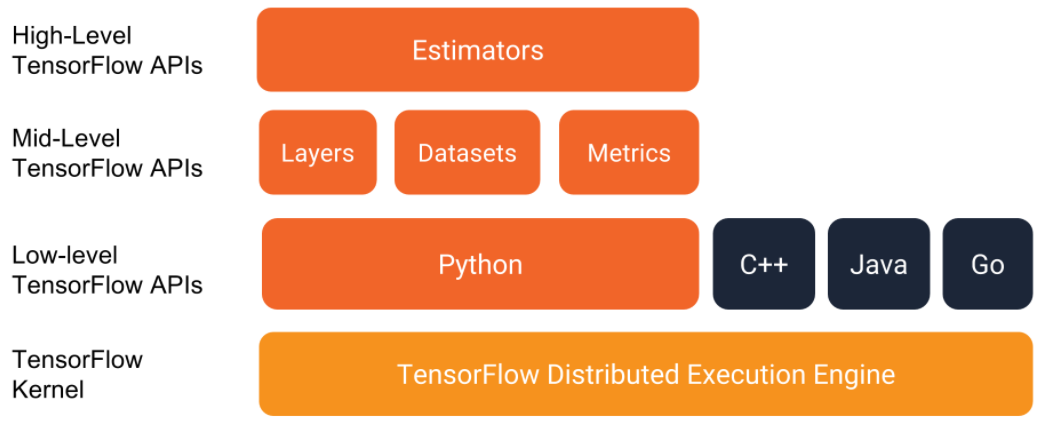
\includegraphics[width=0.3\textwidth]{docu_img_21}
    \caption{Architektur von TensorFlow}
    \label{fig:tf-api}
\end{figure}

Wie Keras und Scikit-Learn bietet auch TensorFlow die Möglichkeit, Verfahren zu verwenden, die leicht zu bedienen sind
und somit keine tiefgehenden Kenntnisse voraussetzen. Darüber hinaus ist es allerdings auch möglich, eigene Modelle und
Strukturen von Grund auf selbst zu definieren und so direkten Einfluss auf das Lernen, Validieren und Vorhersehen zu
nehmen.

\subsubsection{Verwendung von TensorFlow}

In diesem Projekt wurde der Fokus insbesondere auf TensorFlow gelegt. Den elementaren Datentyp von TensorFlow stellen
Tensoren dar. Diese sind mathematisch betrachtet eine Abstraktion von Vektoren und Matritzen. So entspricht ein Tensor
des Typs (0, 0) beispielsweise Skalaren und Tensoren vom Typ (1, 0) Vektoren.
Im Sinne von TensorFlow wird unter einem Tensor\footnote{TensorFlow, tf.Tensor.\newline(https://www.tensorflow.org/api_docs/python/tf/Tensor)}
ein Platzhalter für den Output einer Operation\footnote{TensorFlow, tf.Operation.\newline(https://www.tensorflow.org/api_docs/python/tf/Operation)} verstanden.
Die Besonderheit besteht dabei darin, dass ein Tensor lediglich einen Platzhalter darstellt und keine konkreten Werte
repräsentiert. Der Tensor repräsentiert vielmehr eine Berechnungsvorschrift, nach der sein Output zu berechnen ist.
Auf diese Art und Weise können mehrere Operationen miteinander verkettet werden, die jeweils einen Tensor als Input und
Output haben. Dadurch entsteht ein Graph\footnote{TensorFlow, tf.Graph.\newline(https://www.tensorflow.org/api_docs/python/tf/Graph)},
der demnach eine komplette Berechnung repräsentiert. Sobald diese Berechnung im Rahmen einer Session\footnote{TensorFlow, tf.Session.\newline(https://www.tensorflow.org/api_docs/python/tf/Session)}
ausgeführt wird, \textit{fließt} der Input durch den zuvor definierten Graphen, so dass schlussendlich ein Output
produziert wird.

TensorFlow macht demnach starken Gebrauch des \texit{DataFlow-Paradigmas}\footnote{Wikipedia, Dataflow programming.\newline(https://en.wikipedia.org/wiki/Dataflow_programming)},
wodurch insbesondere die Parallelisierung von Berechnungen erheblich begünstigt wird.

Das Zusammenspiel von Graphen und Sessions kann anhand der nachfolgenden Graphik verdeutlicht werden:

\begin{figure}[h]
    \centering
    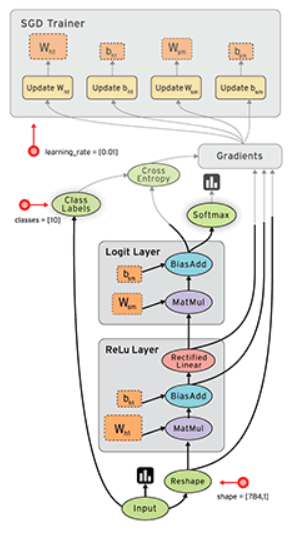
\includegraphics[width=0.3\textwidth]{docu_img_22}
    \caption{Exemplarischer \textit{Dataflow}.}
    \label{fig:tf-api}
\end{figure}

Da im Rahmen des Projekts auf einige Probleme bei der Verwendung von TensorFlow gestoßen wurde, wurde parallel zum
Betrieb von TensorFlow versucht, das Modell mit Keras nachzubauen. Keras ist etwas abstrakter als TensorFlow und bietet
dem Anwender so weniger Konfigurationsmöglichkeiten, wodurch andererseits auch eigene Fehler ausgeschlossen oder eliminiert
werden können.

